\documentclass[../rapport_MVEX01-11-05]{subfiles}
\begin{document}
\section{Statistisk klassificering}\label{sec:klassificering}

Klassificering är ett centralt statistiskt begrepp inom maskininlärning.
Det handlar om att klassificeraren ska göra en kvalificerad gissning för hur
observerad data ska hanteras, baserat på någon typ av ''inlärningsprocess''.
Man skiljer på modellbaserade och modellfria metoder, där de modellbaserade
bygger på modeller av de bakomliggande system som ska analyseras, medan de
modellfria kan ses som mer oberoende av sammanhang.
Man skiljer också på övervakad respektive icke-övervakad inlärning,
där man i det övervakade fallet har etiketter på den träningsdata man stoppar
in, så att man för varje objekt kan säga om det klassificerats rätt eller fel.

Indata till klassificeraren är någon mängd av objekt med någon typ av egenskaper
(features) vilka vi kan mäta. I de givna egenskapernas rum önskar man då
separera objekten i olika kluster. I vissa problem är resultatet binärt,
vilket exempelvis gäller i hudisoleringsproblemet.
I andra fall väljs bland många klasser, vilket gäller gestklassificeringen.
Svårigheten kan förtydligas något med hjälp av figur \ref{fig:kluster}.
\begin{figure}[!htpb]
    \begin{center}
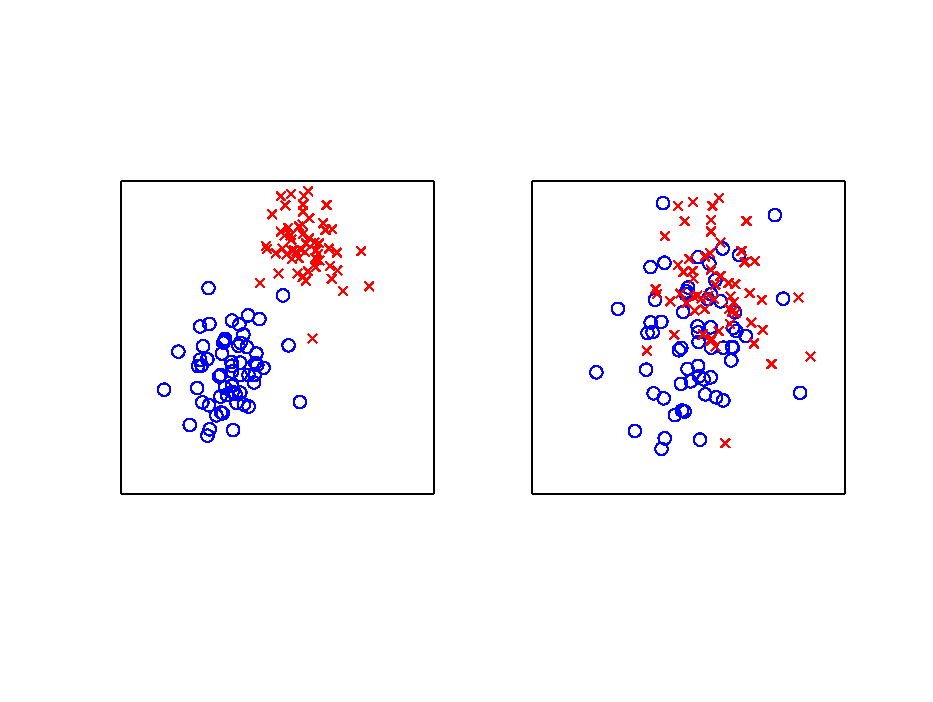
\includegraphics[width=0.8\textwidth,clip=true,trim=2cm 3cm 1.5cm 3cm]{bilder/kluster.pdf}
    \end{center}
    \caption{Det är enkelt att se vart ett objekt hör i den vänstra figuren,
    där de två klasserna är väl separerade. I den högra figuren kan man också se
    skilnad på objekt, men det är nu mycket svårt. Axlarna kan tänkas motsvara
    två godtyckliga egenskaper. I det högra rummet kan man tänka sig två svagare
    egenskaper än i det vänstra. Det kan också motsvara två grupper som
    överlappar varandra i samma rum.}
    \label{fig:kluster}
\end{figure}

Vi kommer att beröra tre klassificerare, två modellfria, i någon mån
prototypbaserade i form av \knn och Gaussian Mixture Models samt en
modellbaserad i avsnittet om dolda Markovmodeller.

%Klassificering handlar om att göra en kvalificerad gissning
%i någon fråga, t.ex.~om en bildpunkt (pixel) innehåller hud, eller om ett område har
%en viss form. I denna mening måste man alltid ha ''träningsdata'' att jämföra med
%till sin
%klassificerare, även om det inte alltid handlar om faktisk träning. Angreppssätt
%så som dolda markovmodeller, random forests, genetiska metoder och liknande kräver
%träning i form av att känd data matas in i klassificeraren varpå denne
%konstruerar en struktur som används för framtida klassificering.
%Enklare metoder så som \knn 
%kräver endast känd data att jämföra med; denna data är då prototypdata.
%
%\notes{Behövs det mer här?}

\end{document} 

